\section{spryVM}
\label{sec:msmmu}

\javier{Points to come across:

\begin{itemize}
  \item Implementation and how it tackles the TLB reach and penalty.
  \item We need figures explaining how the translation works with steps. 
\end{itemize}

}

In this section, we investigate the design space for address translation for MPUs, given the modest associativity requirements and the characteristics of our memory-chip network. Then, we propose and describe our solution, spryVM.

\subsection{Placement}

A straightforward extension of address translation to MPUs integrates an MMU in each MPU. Each MPU probes its MMU on each memory access, and upon a miss in its TLBs, initiates a conventional page table walk. Fig.~\ref{fig:baseline} shows a page walk that references a page table entry residing in another memory chip and partition, which is the common case in systems with multiple chips and partitions. Blue arrows indicate translation-related memory messages, while red arrows show data fetch. %In other words, memory accesses to page table entries are colored in blue, while accesses to page frames are red. 

\begin{figure}[h!]
\centering
 \subfloat[Baseline.]{
  \label{fig:baseline}
%  \includegraphics[width=.32\textwidth,clip,trim = 18mm 213mm 117mm 20mm]{figs/eps/sim-rread-lat.eps}}
   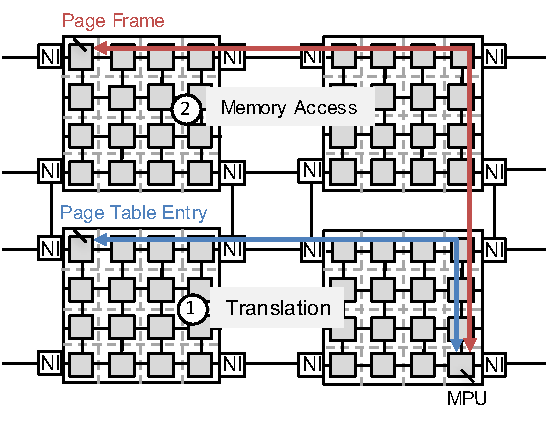
\includegraphics[clip,width=0.75\columnwidth]{figures/floorplan_vanilavm2.pdf}
%   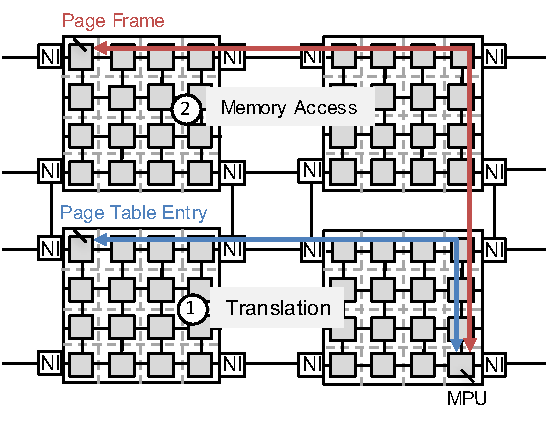
\includegraphics[width=0.69\columnwidth]{figures/floorplan_vanilavm2.pdf}}
   }
%  \hspace{.01in}

 \subfloat[Per-Chip MMU.]{
  \label{fig:chipmmu}
%  \includegraphics[width=.32\textwidth,clip,trim = 18mm 213mm 115mm 20mm]{figs/eps/sim-rread-bw.eps}}
 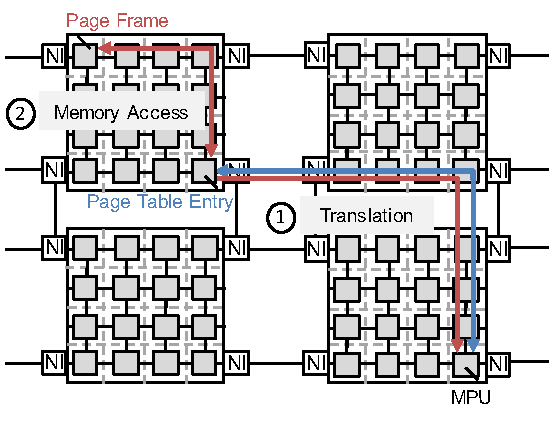
\includegraphics[clip,width=0.75\columnwidth]{figures/floorplan_chipvm2.pdf}
 %  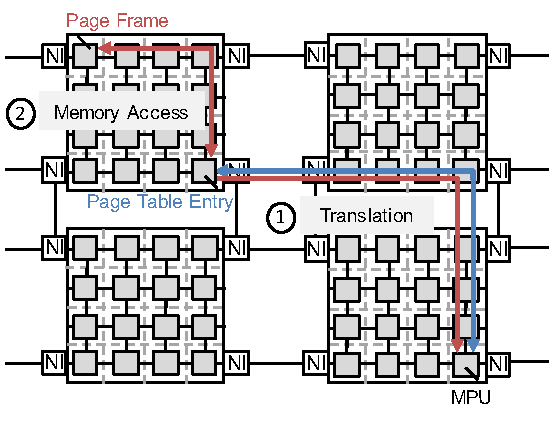
\includegraphics[width=0.69\columnwidth]{figures/floorplan_chipvm2.pdf}}
 }
% \hspace{.01in}

 \subfloat[Per-Partition MMU.]{
  \label{fig:partitionmmu}
%  \includegraphics[width=.32\textwidth,clip,trim = 18mm 213mm 115mm 20mm]{figs/eps/sim-rread-bw.eps}}
 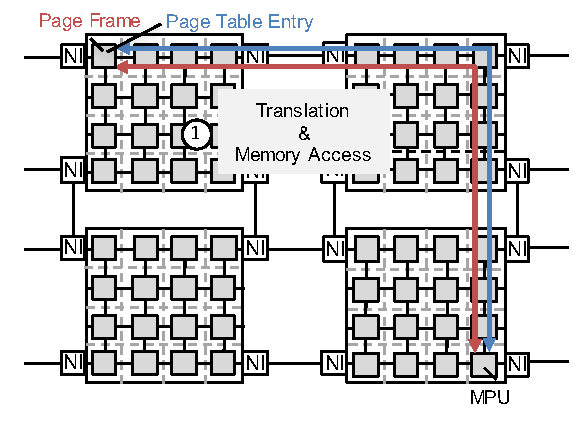
\includegraphics[clip,width=0.75\columnwidth]{figures/floorplan_partitionvm2.pdf}
%  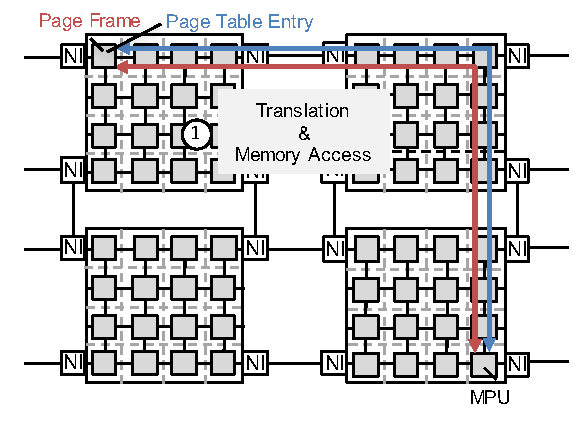
\includegraphics[width=0.695\columnwidth]{figures/floorplan_partitionvm2.pdf}}
 }

\caption{Different translation schemes on 4-chip floor plans. Large squares and small gray squares represent memory chips and partitions, respectively. Translation and memory access messages appear in blue and red, respectively. 
 \label{fig:translationSchemes_comparison}}
\end{figure}

There are several problems with this baseline. First, the page table entry that contains the physical address can be anywhere in the system, involving expensive interconnect traversals which makes page walks costly. Second, the data fetch cannot begin until the translation operation finishes, adding the translation latency to the data fetch latency. Third, the translation process does not finish until the page table entry returns to the MPU, even if the page table entry and the target page frame are in the same chip or memory partition. The fundamental problem is that there is no direct relation between virtual page numbers and page frames, something inherent to fully associative VM. The consequence is that there is no expected correlation between the location of page table entries and page frames, precluding fetching the data before the page table entry returns to the MPU. Although this design makes sense for fully associative VM, it is not optimal for set-associative VM.

We now exploit the modest associativity requirements and consider memory sets that span a memory chip only. A virtual address identifies a memory chip uniquely, and hence we know that the target page frame is somewhere in that chip. Under this constraint, we can utilize a centralized per-chip MMU, along with a page table and a set of TLBs, as shown in Fig.~\ref{fig:chipmmu}. Upon a page walk operation from an MPU, the virtual address is used to access the per-chip MMU. If the translation is not in the per-chip TLBs, a page walk in the memory chip begins. When the page walk finishes, the MMU in the memory chip starts the data fetch immediately, referencing the page frame (which can reside in any of the partitions in the chip). When the data returns to the per-chip MMU, both the page table entry and data return to the MPU. 

This method is an improvement over the baseline for two reasons. First, translation and data fetch overlap the latency on the interconnect to reach the target memory chip, as only the virtual address is used to locate the memory chip. Second, the translation process finishes as soon as the page walk within the memory chip finishes. However, there is room for improvement. As the virtual address only identifies the memory chip, page frames and page table entries can be in any memory partition. This placement creates two problems. First, the centralized per-chip MMU can be located anywhere in the chip, and upon a page walk, the page table entry could be located in a different partition. Second, the target page frame might also be located in another partition. Based on the latency results of Fig.~\ref{fig:e2elat}, the overhead could be significant. 

Going beyond, we can co-locate the page table entries and the page frames in the same memory partition, where memory accesses are faster, and employ a per-partition MMU. In this case, shown in Fig.~\ref{fig:partitionmmu}, memory sets only encompass a memory partition. The locality-aware placement of the MMU delivers the best performance among all. First, the translation and data fetch operations overlap the latency to reach the memory partition---because only the virtual address is used to locate the memory partition. Second, the translation finishes as soon as the page walk within the memory partition finishes, and since the target page frame is within the same partition, the data fetch can begin immediately (without traversing any interconnect).

\subsection{Page Table}
\label{sec:pagetable}

After defining the location of the memory-side MMUs, the next step is to choose a page table. Although there are many page table implementations~\cite{yaniv:hash}, we choose an inverted page table for the following reasons. First, inverted page tables do not need to be dynamically resized, so they are allocated once and pinned contiguously in memory~\cite{jacob:look}. Second, all the processes whose pages map to the partition share the same page table. Finally, when there are no collisions in the inverted page table, page walks only require a single memory access.

One of the key parameters of an inverted page table is the ratio between the number of page frames and page table entries, also called the load factor~\cite{cormen:introduction}. The load factor directly dictates the rate of collisions (i.e., the frequency of two virtual page numbers mapping to the same page table entry). Importantly, given a load factor, the collision rate is not affected by the working set size or access patterns, assuming uniform hashing~\cite{cormen:introduction}. In Fig.~\ref{fig:memref}, we compare a conventional modulo hash to a stronger k-bit XOR folding~\cite{qureshi:fundamental}, to demonstrate the effects of hashing on page table collisions. As we have not seen significant differences in workloads, process counts, and memory size to working set size ratios, we present an average of all the results. The results indicate that an inverted page table with a load factor of $1/4$ and the fold hash function practically removes all collisions. To achieve similar performance with the modulo hash function we would need a load factor of $1/8$. Hence, our design employs an inverted page table with a k-bit XOR folding hash function and load factor of 1/4.  

\begin{figure}
\centering
   \subfloat[Memory references per\\page walk.]{
     \label{fig:memref}
     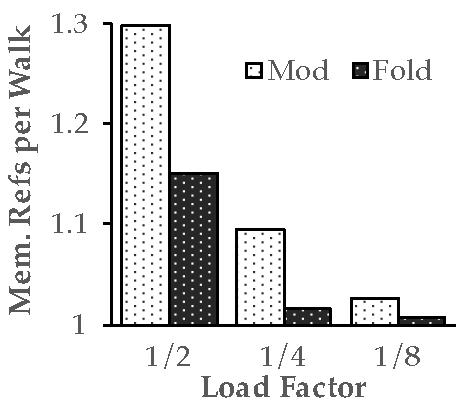
\includegraphics[width=0.45\columnwidth]{graphs/memrefs-bw.pdf}
   }
   \subfloat[Page walk latency normalized to DRAM latency.]{
     \label{fig:pagewalklat}
     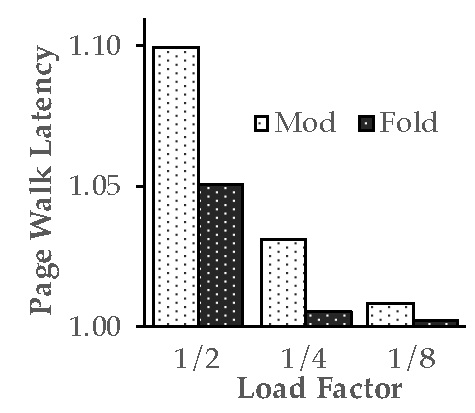
\includegraphics[width=0.45\columnwidth]{graphs/pagewalklat-bw.pdf}
   }
   \caption{Inverted page table performance.}
   \label{fig:IPT_perf_load_hash}
\end{figure}

Fig.~\ref{fig:pagewalklat} shows the page walk latency normalized to the latency of a single DRAM access. The page walk latency is within $1.005\times$ of a DRAM access. The reason the page walk latency does not directly correlate with the number of memory references per walk is that we use open addressing for resolving conflicts~\cite{yaniv:hash}. In open addressing, upon a collision, we probe the next entry in the inverted page table, rather than dereferencing a pointer to a new page table entry, exploiting the locality in the DRAM row buffer~\cite{qureshi:fundamental}, and thus reducing the latency overhead of collisions. Additionally, open addressing removes the pointer per page table entry required to resolve collisions. Each entry in our page table holds a 36-bit virtual page number (VPN), a 12-bit address space identifier (ASID), the 36-bit page frame number (PFN),\footnote{Note that we include the PFN and hence support synonyms.} and 12 bits for page flags, fitting in 16-byte entries. We assume 48-bit virtual and physical address. As we allocate four 16B entries for each 4KB page, due to the 1/4 load factor, the inverted page table consumes a modest $1.6\%$ of the physical memory.  

\subsection{TLB Hierarchy}
\label{sec:tlb}

Although a page walk usually introduces a single additional DRAM access within the memory partition, such accesses are still on the critical path. To minimize this overhead, we employ a TLB hierarchy within the memory-side MMUs to cache frequently used translations. Fig.~\ref{fig:tlb_hitratio} shows how the TLB hit ratio scales as the number of entries increases (more details on the methodology are found in Section~\ref{sec:methodology}). As our translation performance is less dependent on the TLB's hit ratio (due to fast page walks), we average the results across all workloads and scenarios. However, because the memory-side MMUs are shared across all processes in the system (in contrast to conventional MMUs which are bound to a single execution unit), we break down the average results across process counts. Although we expect few processes running concurrently on the MPU cluster,\footnote{A single process can run on an arbitrary number of MPUs.} we see that even with 8 different processes, a TLB with 64 entries, which is the usual size of a first-level TLB, achieves a hit ratio in excess of than $80\%$. Additionally, increasing the number of entries beyond 1024 gives diminishing results, which again matches the size of a conventional second-level TLB. Hence, a conventional two-level TLB hierarchy, a first level with 64 entries and a second level with 1024 is a sound approach. As each MMU integrates its own TLBs, its TLB content does not reflect accesses to others partitions and hence is robust across any memory chip and partition counts.

%All MPUs running in the same address space are a single process

\begin{figure}[t]
   \centering
   %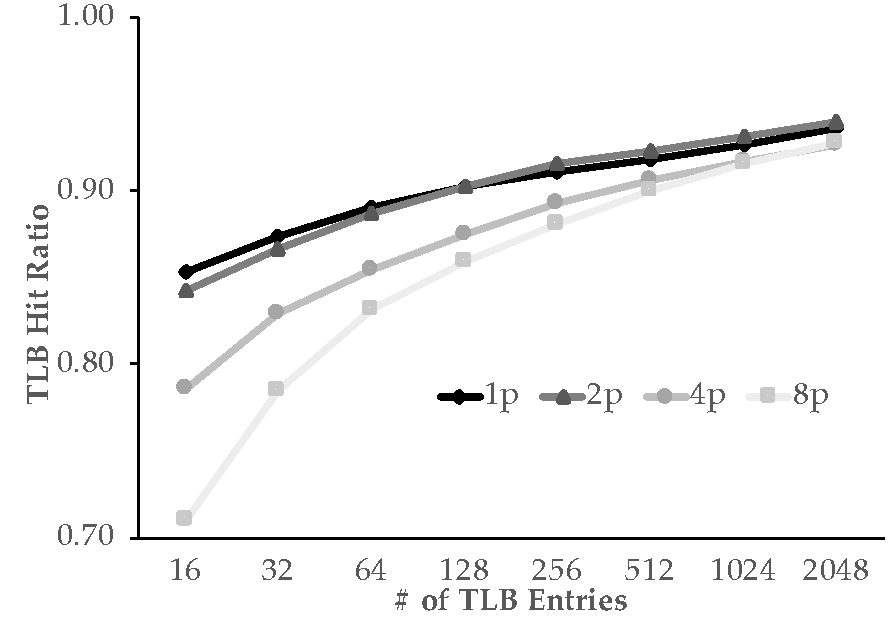
\includegraphics[width=0.8\columnwidth]{graphs/tlbhitratio-marker.pdf}
   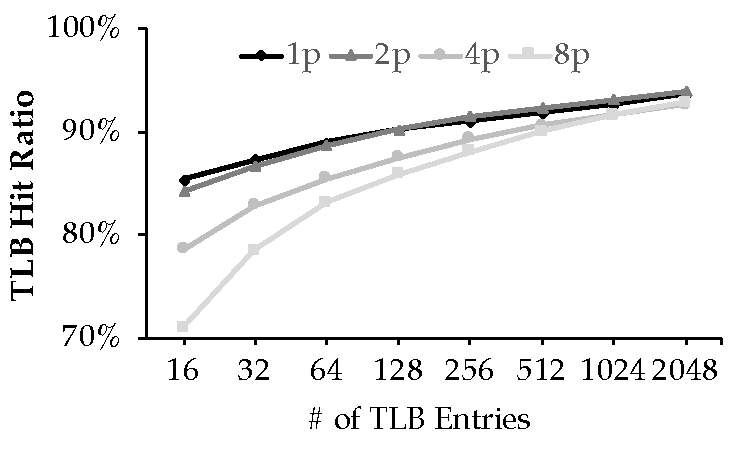
\includegraphics[width=0.8\columnwidth]{graphs/tlbmissratio.pdf}
   \caption{TLB hit ratio sensitivity analysis.}
   \label{fig:tlb_hitratio}
   
\end{figure}

\begin{figure}
\centering

 \subfloat[TLB hit operation.]{
  \label{fig:tlb_hit}
%  \includegraphics[width=.32\textwidth,clip,trim = 18mm 213mm 117mm 20mm]{figs/eps/sim-rread-lat.eps}}
   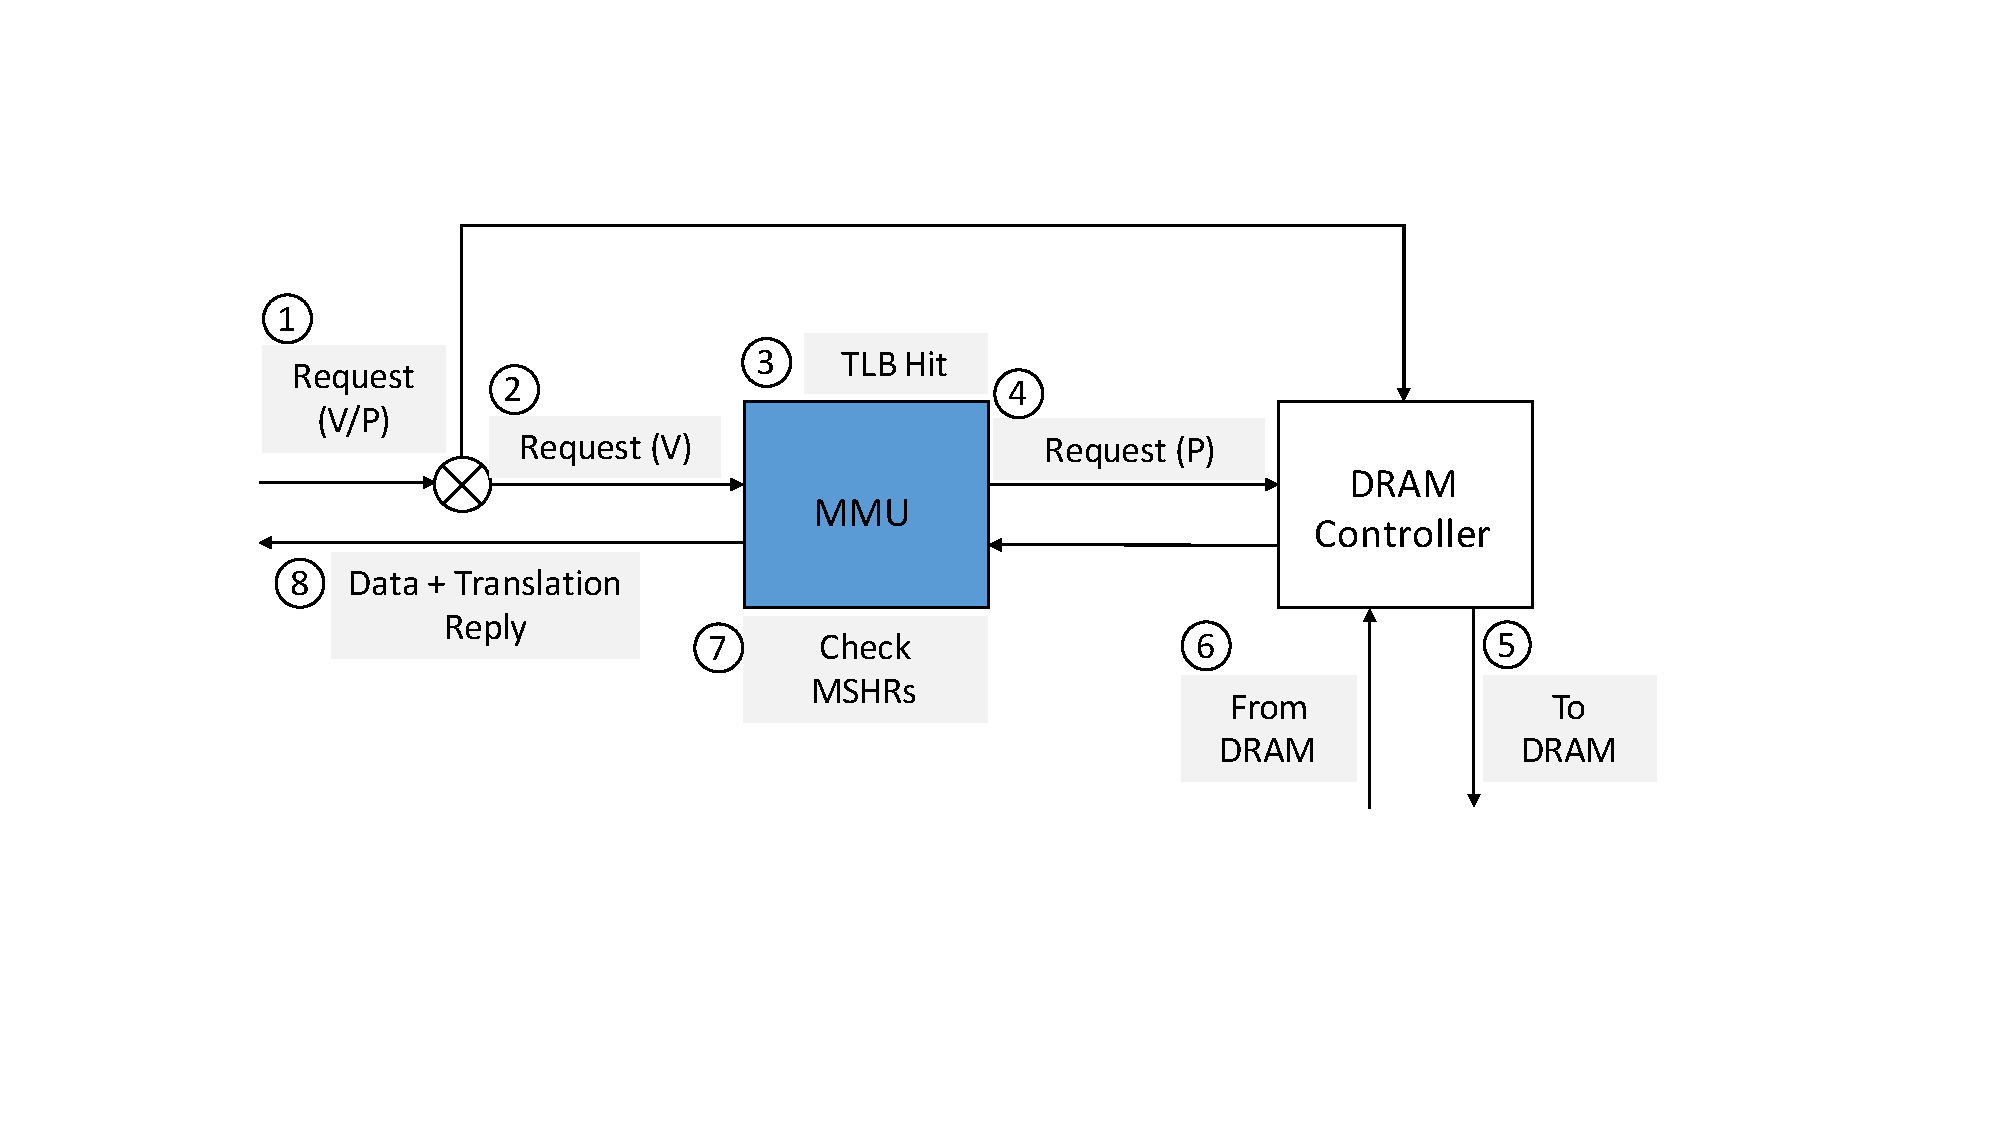
\includegraphics[clip,width=0.95\columnwidth]{figures/hit2.pdf}
   }
   
%  \hspace{.01in}

 \subfloat[TLB miss operation.]{
  \label{fig:tlb_miss}
%  \includegraphics[width=.32\textwidth,clip,trim = 18mm 213mm 115mm 20mm]{figs/eps/sim-rread-bw.eps}}
 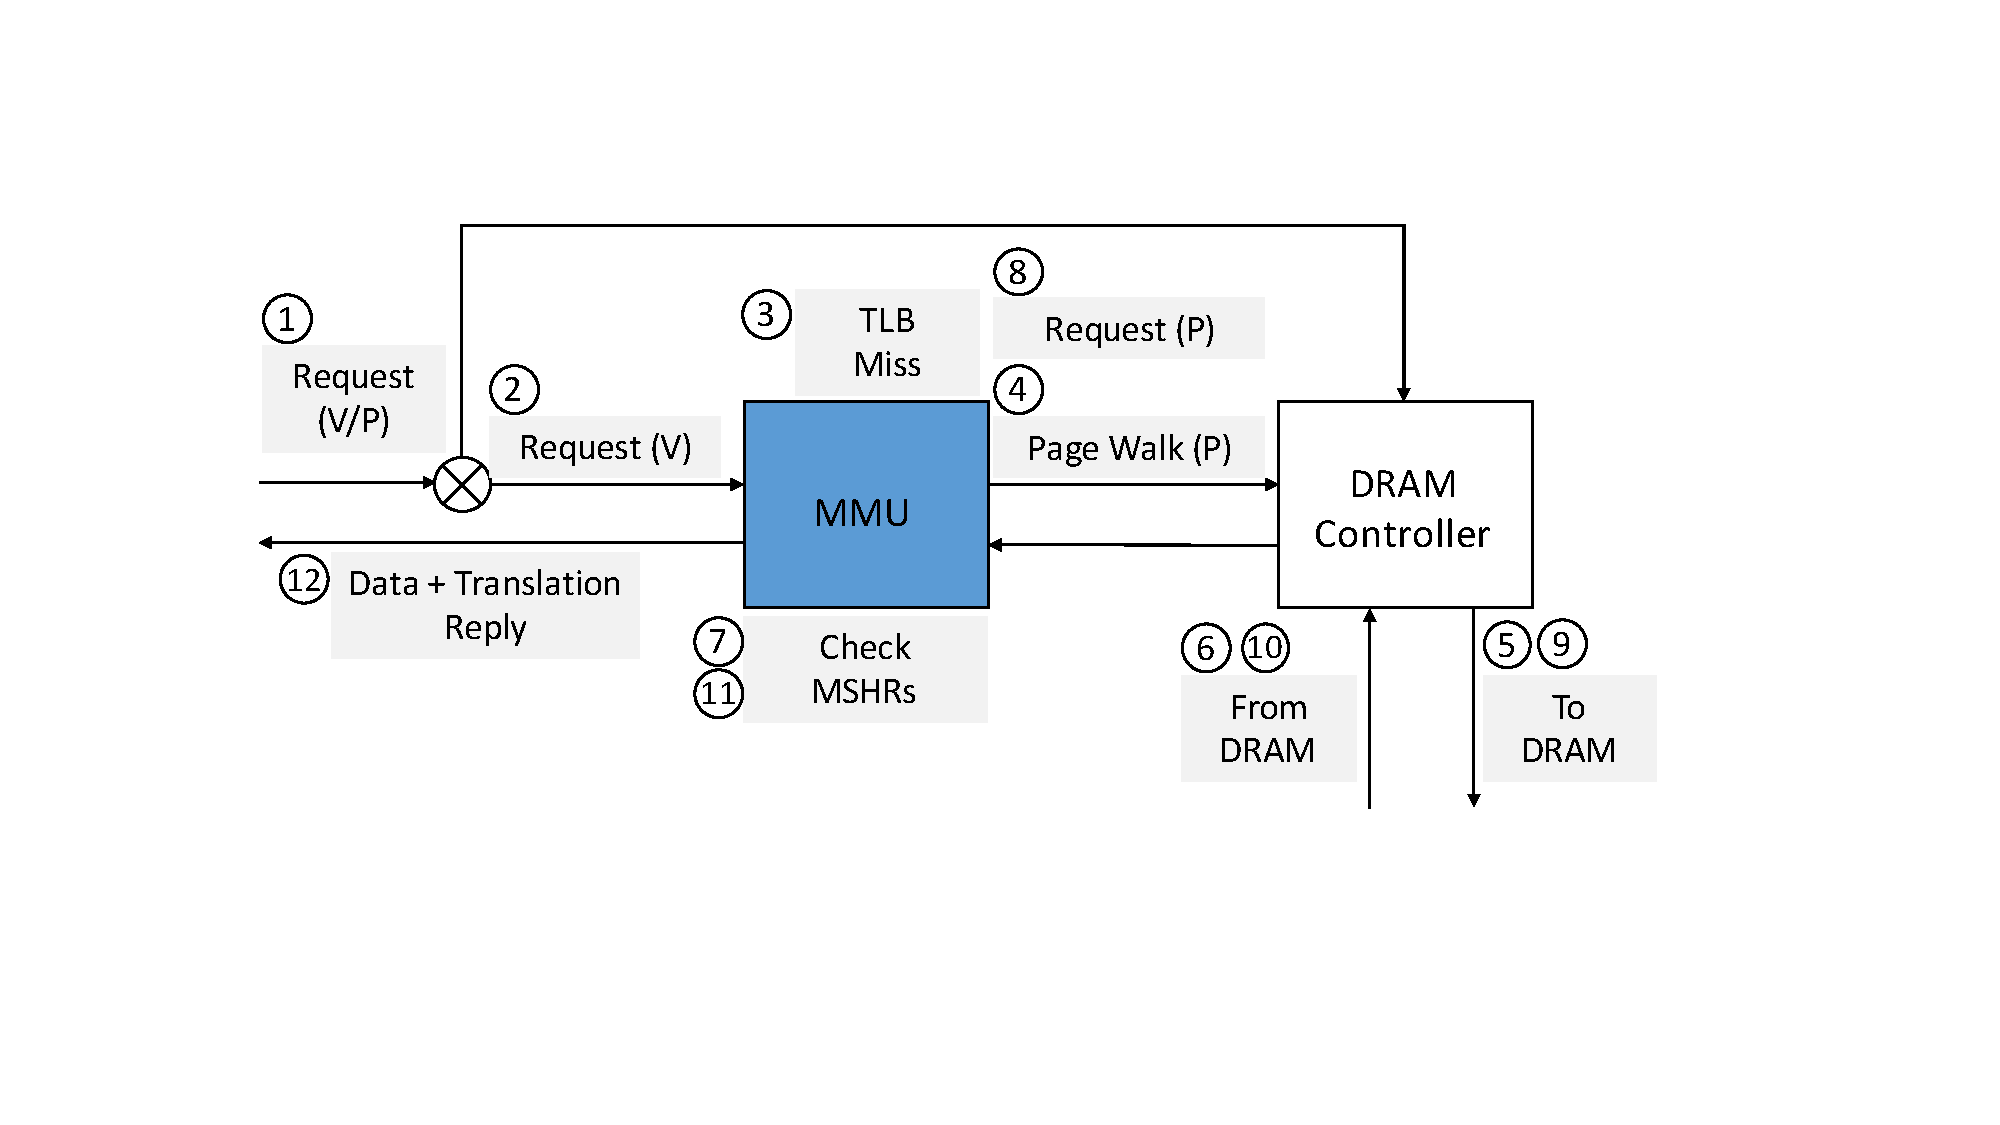
\includegraphics[clip,width=0.95\columnwidth]{figures/miss2.pdf}
 }

\caption{Operation flow of memory-side MMUs.
 \label{fig:tlb_ops}}
 
\end{figure}

\subsection{Putting Everything Together}
Now that we have defined the placement of the MMUs, the page table, and the TLB hierarchy, we provide a walkthrough of the memory-side MMU's operation in Fig.~\ref{fig:tlb_ops}.

In Fig.~\ref{fig:tlb_hit}, we look at the case where the TLBs in the memory-side MMU experience a hit. A request from an MPU arrives at the router of the target partition which forwards it to the MMU (1). A mux checks whether the message uses virtual or physical addresses (2). Memory requests that use physical addresses either come from CPU cores, DMAs, or MPUs that hit in their TLBs.\footnote{MPUs tag requests that use virtual addresses with a cookie.} In the case of physical addresses, the request is sent directly to the DRAM controller. In this example, the request uses virtual addresses, hence arriving at the MMU, and the TLB hierarchy is probed, resulting in a TLB hit (3). Note that the hit requires both the VPN and ASID bits (which are in the request) to match. The MMU then appends the offset bits to the PFN to generate the physical address, creates an MSHR entry tagged with the physical address, and sends a request to the DRAM controller (4). When the DRAM controller finds the address, it sends DRAM commands to fetch the appropriate cache block (5). When the reply comes back (6), the DRAM controller forwards the reply to the MMU, which checks the MSHRs for a match (7). Upon a match, the MMU sends the reply back to the MPU, containing both the data and translation (8).

In Fig.~\ref{fig:tlb_miss}, the memory-side MMU experiences a miss in its TLBs, triggering a page walk. A virtual request from an MPU arrives at the mux (1) and gets forwarded to the memory-side MMU (2). The MMU probes its TLB hierarchy, but the page table entry is not cached (3). The MMU generates the physical address of the page table entry by adding the output of the hash function on the request's virtual address to the base address of the inverted page table. The MMU then creates an MSHR entry tagged with this physical address and sends the request (for the page table entry) to the DRAM controller (4). When the DRAM controller finds the address, it sends DRAM commands to fetch the appropriate page table entry (5). When the reply comes back (6), the DRAM controller forwards the reply to the MMU. The MMU checks the MSHRs for a match (7). The matching MSHR entry indicates that it was a page walk, and hence the MMU generates the request for the actual cache block (8), and repeats the steps shown for the TLB hit operation: (9), (10), and (11). Last, the MMU sends the reply back to the MPU with the data and translation (12). 

Note that most of the functionality of the MSHRs in the MMU is performed by the request queues at the memory controller. We could extend the state of the queues and provide the same functionality. However, we avoid the complexity of extending the memory controller due to the modest hardware requirements for the MSHRs, 64 to 128 entries~\cite{lee:simultaneous} assuming worst-case overprovisioning. Additionally, to further reduce the already low bandwidth requirements of page walks (due to high TLB hit ratios), we indicate to the memory controller that the request for the page table entry is 16 bytes, instead of the conventional 64-byte requests. Existing memory controllers of 3D memories already support requests of different size~\cite{micron:hmc}.


